\chapter{Work Plan}\label{chap:chap3}

\section*{}

The current chapter comprehends the work plan for the dissertation, including its activities and respective time frames.
It will also be explained the datasets that will be used in the project.

\section{Planning}

Given that the preparation phase is already finished, there will be approximately 5 months for the realization of the dissertation.
That corresponds to a time frame between February 2014 and July 2014. In order to complete the dissertation in the given time, it will be given more emphasis to the
prediction of churn users and the prediction of users that continue in the future.

The planning is divided in the four following stages:
\begin{itemize}
  \item Study, selection and testing of algorithms to predict the users that maintain.
  \item Study, selection and testing of algorithms to predict the users that dropout.
  \item Study, selection and testing of algorithms to predict new users.
  \item Writing of the dissertation.
\end{itemize}

%\begin{figure}[h]
  %\begin{center}
    %\leavevmode
    %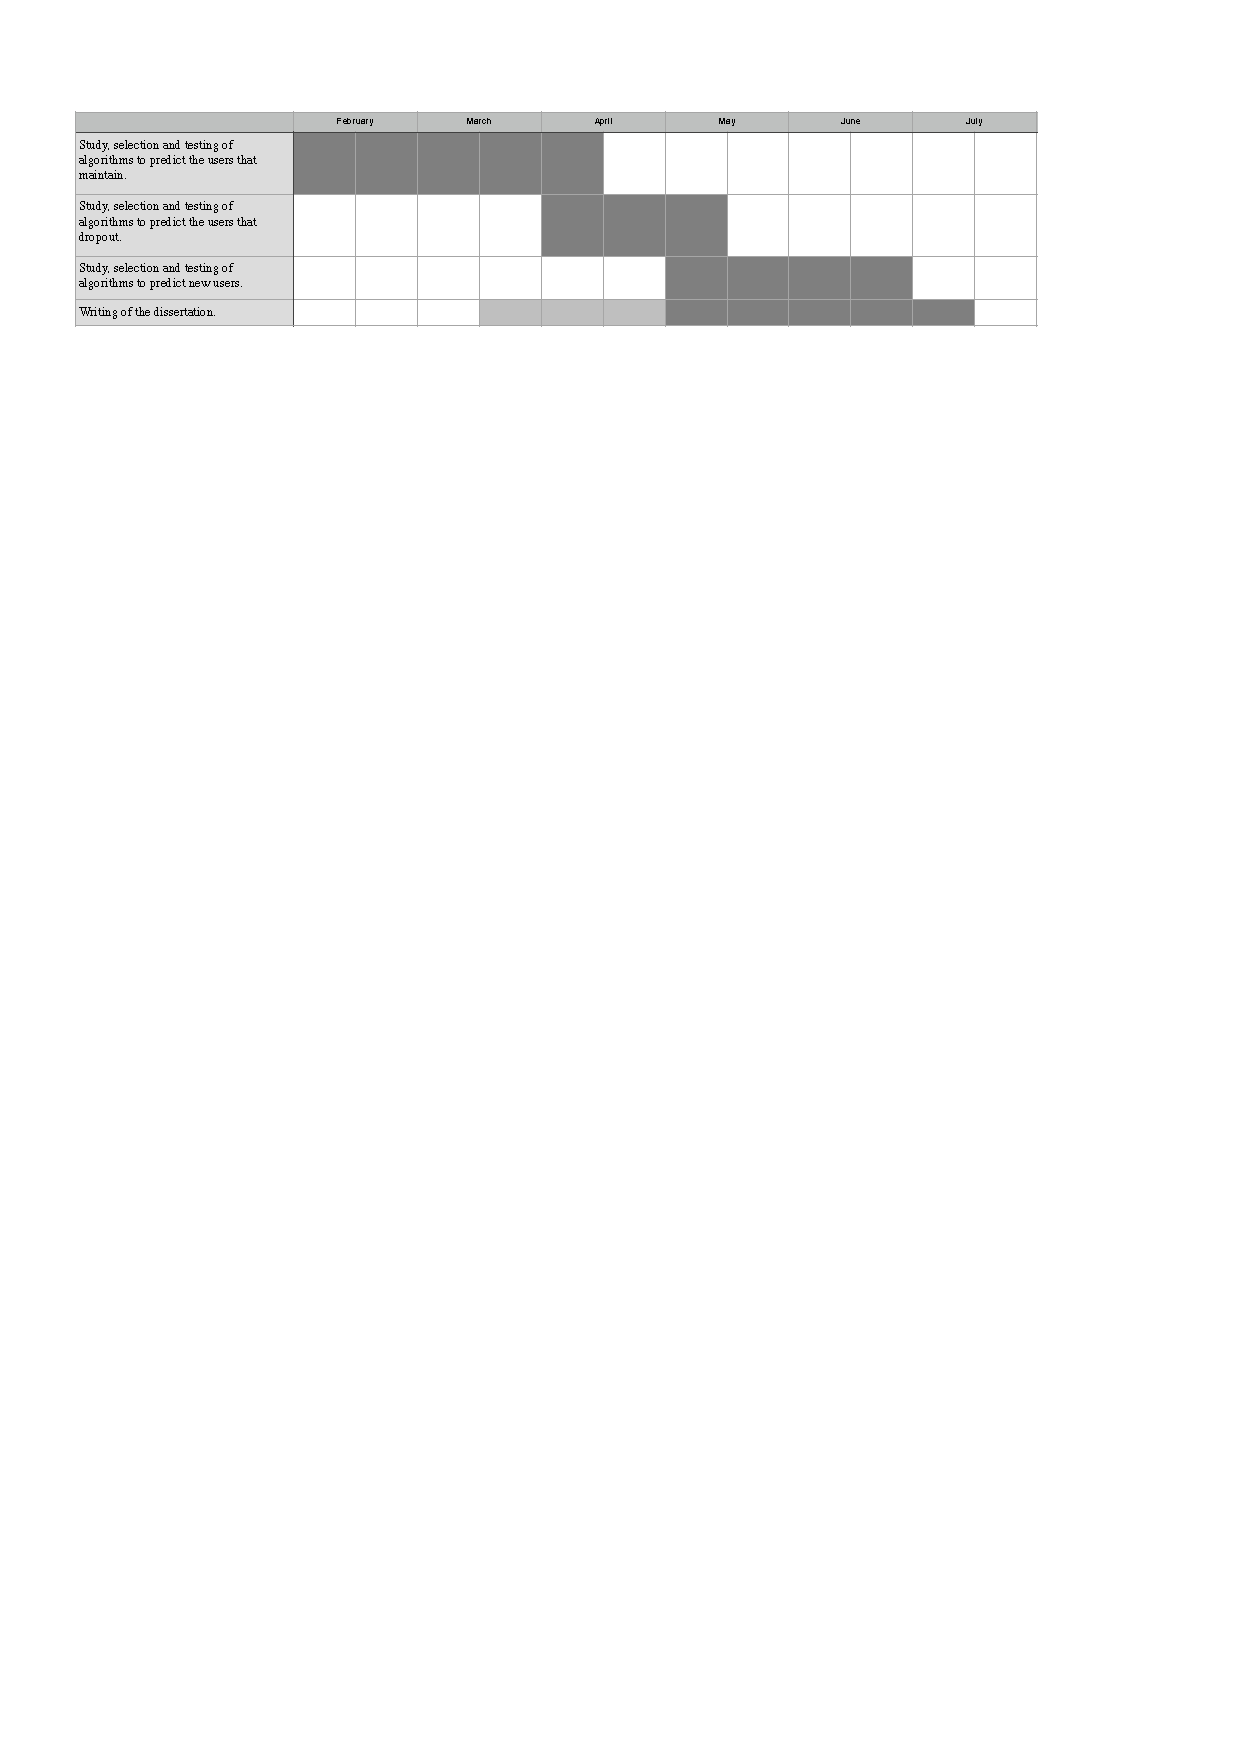
\includegraphics[width=0.96\textwidth]{timeline}
    %\caption{Gantt chart}
    %\label{fig:Timeline}
  %\end{center}
%\end{figure}


\begin{figure}[h]
\begin{center}

\begin{ganttchart}[
    %hgrid,
    %vgrid,
    %x unit=4mm
      y unit title=0.6cm,
      y unit chart=1.5cm,
      x unit=0.8cm,
      vgrid,hgrid,
      title height=1,
      bar/.style={fill=gray!50},
      progress label text={},
      newline shortcut=true,
      bar label node/.append style={align=left},
      bar height=0.4
  ]{1}{12}
    % Time labels
      \gantttitle{2014}{12} \\
      \gantttitle{February}{2}
      \gantttitle{March}{2}
      \gantttitle{April}{2}
      \gantttitle{May}{2}
      \gantttitle{June}{2}
      \gantttitle{July}{2} \\

      % Tasks
      \ganttbar{Study, selection and testing of algorithms\ganttalignnewline
      to predict the users that maintain}{2}{5} \\
      \ganttbar{Study, selection and testing of algorithms\ganttalignnewline
      to predict the users that dropout}{5}{7} \\
      \ganttbar{Study, selection and testing of algorithms\ganttalignnewline
      to predict new users}{7}{10} \\
      \ganttbar{Writing of the dissertation}{7}{12} 
      \ganttbar[bar/.style={fill=gray!20}]{}{4}{7}
\end{ganttchart}

\end{center}
\caption{Gantt Chart}
\end{figure}


%PLANEAR COMO DISTRIBUIR AS FASES e pôr mais lodo em cada uma

\section{Experimental Data}

During the project it will be used multiple datasets from multiple sources containing ad requests. 
Only one will be used at a time. 
An ad request contains a timestamp, an user ID, a location ID and an URL plus a unknown number of
additional parameters, such as, cookies, etc.

\section{Thesis Work Evaluation}

The results will be validate in various different ways:
\begin{itemize}
    \item by comparing the results with real data. For this, analytical methods of error calculation will be used.
    \item by comparing the results with past data copied to the future.
    \item by comparing the results with the tool that Shiftforward uses today.
\end{itemize}
